\section{Statistics for Beginner's Algorithm}
\label{sec:beginnersStat}
In order to get the average length of a solution of beginner's algorithm we must determine how many moves of scrambling must be applied in order to find the highest average number of twists required to solve the \cube{}.
By computing the average for different length of scramble sequences the graph quickly becomes steady at around 40 scrambles with 10.000 tested \cube{}s (see figure \ref{fig:beginnersScramble} and appendix \ref{chap:beginnerResults}). To be sure that we get a good result we will use 50 scrambles in the next tests.
\begin{figure}[htbp]
	\centering
		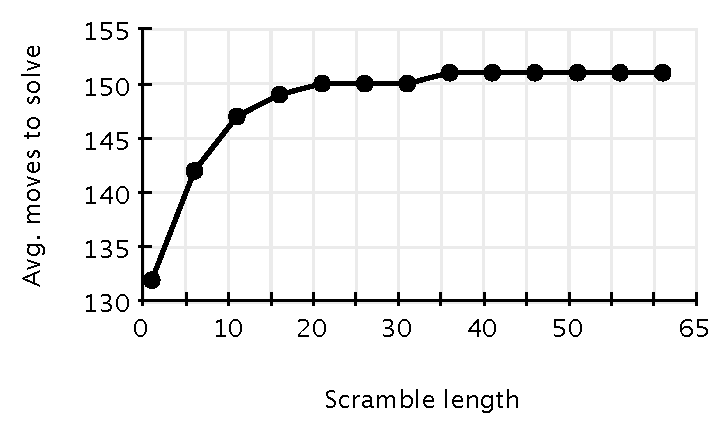
\includegraphics[scale=0.6]{input/pics/beginnersScramble.pdf}
	\caption{\myCaption{The graph shows the amount of moves needed to solve a cube with x scrambles. The lines are only for visual effect and do not represent the average between the points.}}
	\label{fig:beginnersScramble}
\end{figure}

Now that the length of the needed scramble sequence is determined the average number of \twist{}s needed to solve the \cube{} can be found.
%By scrambling 10 million \cube{}s and solve them with the beginner's algorithm we get an average of 151 moves.
By scrambling and solving 10 millions \cube{}s with our implementation of beginner's algorithm an average of 151 \twist{}s is obtained.
A test using only 1 million \rubik{}s is run three times in order to ensure that the test is reliable.
This test also showed an average of 151 moves in every run, meaning that this result is reproducible.
The raw data from both tests can be found in appendix \ref{chap:beginnerResults}.
%Which is the average of beginner's algorithm.

The maximum length of the solution is 241 moves and the minimum length is 56 moves.
The average time spent on each solve was:
\[
\frac{502552 \text{ ms} + 490385 \text{ ms} + 498937 \text{ ms} + 4734126 \text{ ms}}{10^{7} + 3 \cdot 10^{6}} = 0.478923077 \text{ ms}
\]

The data was gathered on a computer operated by Windows 7 64 bits running on a 2.5 GHz AMD Quad Core processor (905e) with 4 GB DDR-3 RAM.

A peculiar note is that with a scramble of length one, the algorithm needs an average of 132 moves with a maximum of 155 and a minimum of 94 moves to solve it again.
This illustrates the twist-wise inefficiency of this algorithm very well.